
\documentclass[conference]{IEEEtran}
\usepackage[utf8]{inputenc}
\usepackage[spanish]{babel}
\usepackage{amsmath}
\usepackage{amsfonts}
\usepackage{amssymb}
\usepackage{graphicx}

\usepackage{tabularx}
\usepackage{booktabs}
\usepackage{siunitx}
\usepackage{multirow}

\usepackage{fancyhdr}
\cfoot{\thepage}

\ifCLASSINFOpdf
 
\else
  
\fi


\hyphenation{op-tical net-works semi-conduc-tor}


\begin{document}


\title{Mezcladores de Radiofrecuencia}



\author{
\begin{tabular}{cccc}
\Large Gallo, Facundo &\Large Guazzaroni, Luca &\Large  Nievas, Martin &\Large Viel, Nahuel \\ 
63579 & 62630 & 61997 & 61999 \\ 
facundogallo01\makeatletter @gmail.com & lucaguazzaroni\makeatletter @gmail.com & martin.nievas.ar\makeatletter @gmail.com & nahuviel\makeatletter @gmail.com \\ 
\multicolumn{4}{c}{\bf Univesrsidad Tecnólogica Nacional - facultad regional córdoba}\\\\ 
\end{tabular} 
}
        
\maketitle

% As a general rule, do not put math, special symbols or citations
% in the abstract

\IEEEpeerreviewmaketitle

\section{Introducción} 
En el campo de las telecomunicaciones, un mezclador es un circuito no lineal variante con el tiempo o un dispositivo capaz de mezclar dos señales de entrada, de  frecuencias  f1  y  f2 respectivamente, produciendo a su salida una mezcla de señales, frecuencias  $mf1+  nf2$, donde  $m$  y  $n$  son números enteros, siendo las frecuencias más deseables $f1 + f2$ y $f1 - f2$ si $f1 > f2$ o viceversa.

Cualquier dispositivo alineal puede ser un mezclador, diodos, transistores bipolares,  FETs, etc. La no linealidad  es necesaria  para  producir  nuevas  frecuencias.  La  elección  del  dispositivo  y  del  circuito  depende  de  las  consideraciones  que  se  realicen  sobre  la  ganancia  o  pérdida  de  conversión,  rango  dinámico,  ancho  de  banda, figura de ruido,  aislación entre los puertos, generación de frecuencias indeseables, costo, y adaptación de sus puertos.
\section{Teoría básica de los mezcladores}
La Fig. \ref{mezc1} ilustra un mezclador sencillo formado por un dispositivo no lineal con dos voltajes de entrada $v1(t)$ y $v2(t)$ de diferentes frecuencias $f1$ y $f2$, respectivamente. Si el dispositivo fuera perfectamente lineal, el voltaje o corriente de salida contendría sólo las frecuencias $f1$ y $f2$. La naturaleza no lineal determina qué otras frecuencias se generan.
		
\begin{figure}[h!]
\centering
\includegraphics[scale=0.8]{Imagenes/mezc1.eps}
\caption{Dispositivo no lineal usado como mezclador.}
\label{mezc1}
\end{figure}
En general, la relación entrada-salida en el dominio del tiempo se puede expresar por la serie de Taylor
\begin{equation}
i_{0}(t) = I_{0}+ a\cdot v_{i}(t) + b\cdot [v_{i}(t)]^2 + c\cdot [v_{i}(t)]^3 + \ldots
\label{eq:1}
\end{equation}
donde $I_o$ es la corriente de salida en reposo y $v_{i}(t)$ representa la suma de los efectos de todas las señales de entrada.

Si la entrada contiene sólo una frecuencia, la no linealidad generará armónicas de esta frecuencia y alterará la componente de CC.\\
Si se tienen varias frecuencias de entrada, se generarán frecuencias suma y diferencia, así como armónicas. Las frecuencias de suma y diferencia generadas por el término cuadrático en \eqref{eq:1} se llaman productos de intermodulación de segundo orden; las originadas por el término cúbico, productos de tercer orden.

Un dispositivo de ley cuadrática es ideal para servicio de mezclador, pues se produce el número mínimo de frecuencias indeseables, si el dispositivo tiene buena característica de transferencia.
			
\section{Terminología de los mezcladores}
\subsection{Pérdida de conversión}
Podemos considerar que el parámetro  más importante de un mezclador es la pérdida de conversión. La misma se define como la diferencia entre la potencia de RF de entrada y la potencia de IF de salida (Fig. \ref{per1}).\\
$$CL = P_{RF} - P_{IF} $$

			\begin{figure}[h!]
			\centering
			\includegraphics[scale=0.4]{Imagenes/per1.eps}
			\caption{Definición gráfica de pérdida por conversión.}
			\label{per1}
			\end{figure}

\subsection{Pérdidas de asilación}
La  aislación  es  una  medida  de  la  cantidad  de  potencia  que  se  fuga   o  filtra  de  un  puerto  a  otro  puerto  del mezclador. La aislación se obtiene por balanceo del mezclador, tanto de los elementos lineales del circuito, como el  apareamiento  de  los  diodos o transistores, o por el uso de dispositivos unilaterales. Sin embargo, siempre existe alguna pequeña cantidad de potencia de pérdida entre los puertos de RF, LO y IF. 

La  aislación  es  la  diferencia  de  potencia  entre  la  entrada  de  señal  en  un  puerto  y  la  potencia  de la misma frecuencia fugada a otro puerto, tal como vemos en la Fig. \ref{per2}.
			
			\begin{figure}[h!]
			\centering
			\includegraphics[scale=0.4]{Imagenes/per2.eps}
			\caption{Definiciones de las aislaciones de un mezclador, de izquierda a derecha LO-RF, LO-IF y RF-IF.}
			\label{per2}
			\end{figure}

\subsection{Pérdida por compresión}
En  condiciones  de  funcionamiento  normal,  la  pérdida  de  conversión  del  mezclador  será  constante, independientemente  de  la  potencia  de  entrada  RF.  Si  las  potencia  de  entrada  de  RF  se  incrementa  en  1  dB, entonces la salida de potencia de FI de potencia también se incrementará en 1 dB (la diferencia es la pérdida de conversión). Sin embargo,  cuando  la potencia de RF se vuelve demasiado grande esta regla no se cumple. El punto  de  1  dB  de  compresión  es  una  medida  de  la  linealidad  del  mezclador  y  se  define  como  la  entrada   de potencia de RF necesaria para aumentar la pérdida de conversión en 1 dB  del valor ideal. Esto se muestra en la Fig. \ref{per3}:
			
			\begin{figure}[h!]
			\centering
			\includegraphics[scale=0.5]{Imagenes/per3.eps}
			\caption{Representación gráfica del punto de compresión de 1 dB.}
			\label{per3}
			\end{figure}

En  condiciones de funcionamiento lineal, la potencia LO es mucho más fuerte   que la potencia de RF por lo que la acción de conmutación de  los  diodos  está  totalmente dominada  por el  LO.  Sin embargo, en la compresión, la potencia  de  RF  compite  con  la  potencia  del  LO  por  lo  que  la  acción  de  conmutación  de  los  diodos  se  ve 
comprometida.

Un  funcionamiento  del  mezclador  en  condiciones  de  compresión  incrementa  los  niveles  de  distorsión  por intermodulación y aumenta la perdida de conversión.

\subsection{Figura de ruido}
La figura de ruido de un mezclador es aproximadamente igual que la pérdida de conversión, salvo en los casos donde se utilicen diodos con gran figura de ruido. Cuando se eligen mezcladores para aplicaciones de pequeña señal, como el caso de un receptor sin amplificador de RF, es conveniente seleccionar un mezclador con una pérdida de conversión tan baja como sea posible.
			

\section{Tipos de mezcladores}
Construyendo el mezclador con un número par de dispositivos dispuestos en forma simétrica es posible eliminar, o atenuar considerablemente, algunas frecuencias o armónicos de las señal aplicada en un terminal en el otro. Es decir, mejoramos notablemente la aislación.

No es conveniente que la señal del oscilador local (LO) aparezca en el terminal de frecuencia intermedia (IF) ni en el terminal de radio  frecuencia (RF), como tampoco  es conveniente  que  la  señal  de  RF  pase  al  terminal  de  IF.

Podemos clasificar a lo mezcladores por el balanceo o equilibrio que emplean.

\begin{enumerate}
	\item de terminación única.
	\item de balanceo simple.
	\item de balanceo doble.
\end{enumerate}

%Cumpliendo con las condiciones impuestas para el desarrollo del práctico, se utilizarán mezcladores para una configuración de un receptor superheterodino de FM (88-108 MHz, IF:10,7 MHz) con una potencia de LO: 8 dB y de RF:-10 dB, para una carga de 50 $\Omega$.
%
%Se podrá observar que en la construcción de los mezcladores existen 2 filtros pasabanda, se utilizaron filtros de cuarto orden del tipo Chevyschev, se eligió éste modelo por su característica de tener una pendiente abrupta y poder así que solo pase la frecuencia necesitada. Uno en la parte de IF para poder recuperar la componente espectral que a mi me interesa que será la de 10,7 MHz y también se observa la presencia de un filtro en la entrada de RF, éste tiene como objetivo dejarme pasar el canal de FM y no así armónicos que no me interesan. 

\subsection{Mezclador de terminación única}
Son aquellos mezcladores que usan un único dispositivo alineal, que puede ser un diodo o un transistor. Debido a que solo poseen un dispositivo alineal, no hay  simetrías que permitan eliminar frecuencias no deseadas en alguno de los terminales mediante la cancelación de fase. Sin embargo en aplicaciones  no  muy comprometidas con la supresión de señales indeseadas, el uso de  esta configuración  es totalmente aceptable. 


\subsubsection{Mezclador de terminación única a diodo}
			
			\begin{figure}[h!]
			\centering
			\includegraphics[scale=.5]{Imagenes/terminacion_unica/teminacion_unica_sch.png} 
			\caption{Mezclador de terminación única con un solo diodo.}
			\label{esq1}
			\end{figure}

En la Fig. \ref{esq1} se muestra un circuito de terminación única. La característica fuertemente alineal del diodo permite que solo circule corriente por él cuando la tensión de la señal es mayor que la tensión umbral del mismo.
 
La  característica  no  lineal  del  diodo  es  la  que  origina  nuevas  componentes  de  frecuencia  en  la  corriente  del mismo y por ende en la salida de FI, que es el objetivo perseguido. Se eligió una frecuencia de RF de 98 MHz, a la cuál la frecuencia del LO es de 108,7 MHz (Fig. \ref{LO_termUnica}). El diodo será el encargado de generar  el producto intermodulación de éstas dos frecuencias, y con el filtro poder recuperar la componente espectral que se desea la cual será la resta de los mismos 
$$ f_{IF} = f_{LO} - f_{RF} = 10,7 MHz. $$

\begin{figure}[h!]
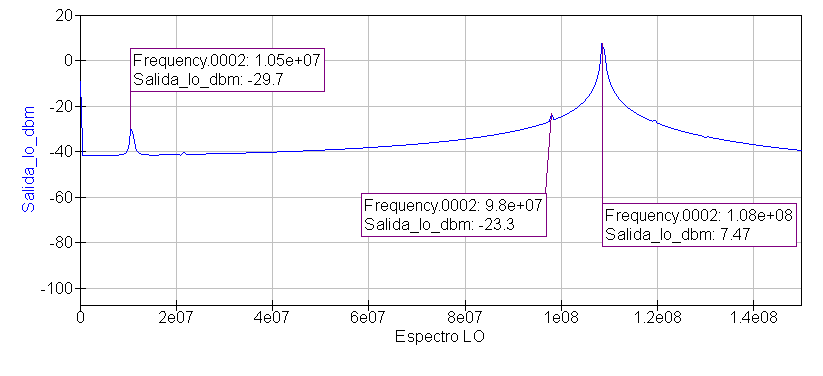
\includegraphics[width= 0.45 \textwidth]{Imagenes/terminacion_unica/Espectro_LO_Aislacion_Term_Unica.png}
\caption{LO en el dominio de la frecuencia en el mezclador de terminación única.}
\label{LO_termUnica}
\end{figure}

En la Fig. \ref{RF_termUnica} se presentan el espectro en frecuencia del puerto de RF, se puede distinguir que aparece la componente espectral de LO y de IF, esto se debe a que no hay una buena aislación entre puertos. Al tener LO mas potencia que la RF, la componente de LO en RF será de mayor amplitud que la RF misma.

\begin{figure}[h]
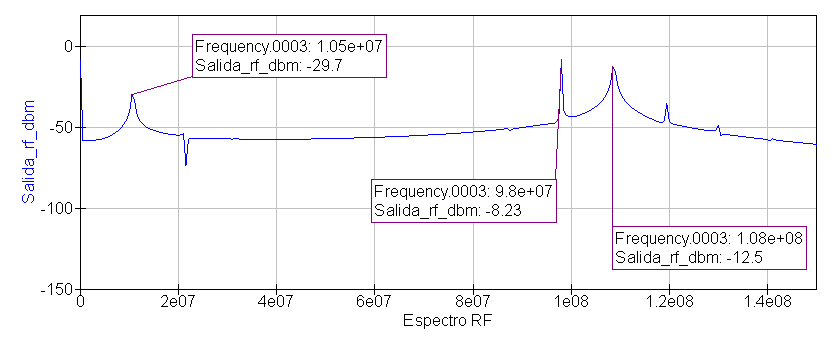
\includegraphics[scale=.4]{Imagenes/terminacion_unica/Espectro_RF_Aislacion_Term_Unica.png} 
\caption{Espectro de frecuencia en la entrada del mezclador terminación única}
\label{RF_termUnica}
\end{figure}

\begin{figure}[h]
\includegraphics[scale=.4]{Imagenes/terminacion_unica/Espectro_FI_Aislacion_Term_Unica.png} 
\caption{Salida del mezclador terminación única en el dominio de la frecuencia}
\label{FI_termUnica}
\end{figure}

Analizando la salida (Fig. \ref{FI_termUnica}), se espera obtener solo la señal de IF. Gracias a la presencia de un filtro se logra eliminar todas las intermodulaciones indeseadas, quedando solo la IF, con una potencia notablemente pequeña. La IF resultante, al tener poca amplitud, exigirá que el amplificador a utilizar en una etapa posterior, tenga una ganancia bastante grande, lo que implicará un gran costo.
Los valores de aislación pueden observarse en el cuadro (\ref{terminacionUnica})

\begin{table}[h!]
  \begin{tabular}{SSSSSS}
    \toprule
      \multicolumn{6}{c}{Pérdidas por aislación [dB] mezclador terminación única} \\
      \midrule
    \tiny $LO-IF$&\tiny$IF-LO$&\tiny$RF-IF$&\tiny $IF-RF$&\tiny $LO-RF$&\tiny $RF-LO$\\
		\midrule
		75,5 & 1,9 & 57,9 & 1,9 & 20,5 & 13,3 \\
    \bottomrule
  \end{tabular}
  \caption{Valores Terminación única}
  \label{terminacionUnica}
\end{table}

 
\begin{table}[h!]
  \begin{tabular}{SSSSSS}
    \toprule
      \multicolumn{3}{c}{Pérdidas}\\
      \midrule
      \multicolumn{1}{c}{Compresión [dB]}&\multicolumn{1}{c}{Conversión [dB]} &\multicolumn{1}{c}{Figura de Ruido}\\
      \midrule
		3 & 17,8 & 17,8\\
    \bottomrule
  \end{tabular}
  \caption{Valores Balanceo doble}
  \label{tablaTerminacionUnica}
\end{table}

\subsection{Mezclador de balanceo simple}
Usa un número par de dispositivos  alineales, normalmente diodos o FETs, dispuestos en forma equilibrada, de tal manera que el terminal de entrada queda aislada de los otros terminales. En el circuito de la Fig. \ref{balanceoSimple} se observa que el terminal aislado es el de LO. Que un terminal esté aislado implica que una señal aplicada al mismo, por si sola, no produce efecto en los otros terminales. 
En este caso se utilizó una frecuencia de RF de 98 MHz, en el centro del rango de FM. Siendo ésta la frecuencia de RF, el LO interno tendrá que tener una frecuencia de 108,7 MHz, para cumplir con el receptor superheterodino. 
			
			\begin{figure}[h]
			\centering
			\includegraphics[scale=.31]{Imagenes/balanceo_simpmle/balanceo_simple_sch.png} 
			\caption{Mezclador de balanceo simple.}
			\label{balanceoSimple}
			\end{figure}

			\begin{figure}[h]
			\centering
			\includegraphics[scale=.2]{Imagenes/balanceo_simpmle/mezclador_balanceo_simple_salida.png} 
			\caption{Salida del Mezclador de balanceo simple.}
			\label{balanceoSimple_salida}
			\end{figure}


Si se observa la salida (Fig. \ref{balanceoSimple_salida}), la potencia que tiene la IF es mayor en comparación con el mezclador de terminación única. Ésta es una ventaja de esta configuración por sobre la de un solo diodo. Sin embargo la potencia de salida de IF sigue siendo pequeña, lo cuál conlleva a una figura de ruido mala. Como se ve en la Fig. \ref{balanceoSimple} esta configuración también posee un filtro en el puerto de IF que dejará pasar la componente de frecuencia intermedia requerida. Otro aspecto importante es que la aislación mejora notablemente, como podemos observarlo en la Fig. \ref{balanceoSimple_RF} y en la Fig. \ref{balanceoSimple_LO}

			\begin{figure}[h]
			\centering
			\includegraphics[scale=.2]{Imagenes/balanceo_simpmle/mezclador_balanceo_simple_RF.png} 
			\caption{Espectro de frecuencia en la entrada del mezclador de balanceo simple.}
			\label{balanceoSimple_RF}
			\end{figure}


			\begin{figure}[h]
			\centering
			\includegraphics[scale=.2]{Imagenes/balanceo_simpmle/mezclador_balanceo_simple_LO.png} 
			\caption{Espectro de frecuencia en el oscilador local del mezclador de balanceo simple.}
			\label{balanceoSimple_LO}
			\end{figure}

Con los valores de las gráficas anteriores y con los datos de la Fig. \ref{balanceoSimple_compresion}, calculamos las pérdidas por aislación,  las cuales se muestran en el cuadro (\ref{tablaBalanceSimple}) y las pérdidas por compresión y conversión en la tabla \ref{tablaBalanceoSimple_conversion}\\


\begin{table}[h!]
  \begin{tabular}{SSSSSS}
    \toprule
      \multicolumn{6}{c}{Pérdidas por aislación [dB] mezclador balanceo simple} \\
      \midrule
    \tiny $LO-IF$&\tiny$IF-LO$&\tiny$RF-IF$&\tiny $IF-RF$&\tiny $LO-RF$&\tiny $RF-LO$\\
		\midrule
		139 & 18,8 & 137 & 10,7 & 72 & 39,8 \\
    \bottomrule
  \end{tabular}
  \caption{Valores Balanceo simple}
  \label{tablaBalanceSimple}
\end{table}


\begin{table}[h!]
  \begin{tabular}{SSS}
    \toprule
      \multicolumn{3}{c}{Pérdidas}\\
      \midrule
      \multicolumn{1}{c}{Compresión [dB]}&\multicolumn{1}{c}{Conversión [dB]} &\multicolumn{1}{c}{Figura de Ruido}\\
      \midrule
		-4.5  & 58,3 & 58,3 \\
    \bottomrule
  \end{tabular}
  \caption{Valores Balanceo Simple}
  \label{tablaBalanceoSimple_conversion}
\end{table}

			\begin{figure}[h!]
			\centering
			\includegraphics[scale=.6]{Imagenes/balanceo_simple.eps} 
			\caption{Pérdida por compresión en amplificador balanceo simple }
			\label{balanceoSimple_compresion}
			\end{figure}



\subsection{Mezclador de balanceo doble}

En esta configuración, todos los terminales están aislados entre si mediante los dos transformadores, por lo que las frecuencias de las señales de entrada no aparecen a la salida. En la Fig. \ref{balanceoDoble_sch} se observa un mezclador de éste tipo. Cuando la amplitud de LO es positiva conducen los diodos D1 y D2 y cuando es negativa los D3 y D4, de esta forma se evita que componentes de LO aparezcan en otros puertos. Para conseguir una buena eficiencia en este circuito, es necesario que la implementación del puente sea equilibrado, para así obtener un perfecto bloqueo de una señal a otra. 

			\begin{figure}[h!]
			\centering
			\includegraphics[scale=.15]{Imagenes/balanceo_doble/balanceo_doble_sch.png} 
			\caption{Mezclador de balanceo doble.}
			\label{balanceoDoble_sch}
			\end{figure}


			
			
Como se observa en la Fig. \ref{balanceoDoble_salida}, no se encuentra presente la componente LO en la salida, ni aparece en el puerto de RF, esto se debe a que con el puente de diodos equilibrado y ambos transformadores, es muy difícil que una componente de un puerto se acople en el otro, consiguiéndose una asilación casi excelente.
			\begin{figure}[h!]
			\centering
			\includegraphics[scale=.25]{Imagenes/balanceo_doble/balanceo_doble_salida.png} 
			\caption{Salida mezclador de balanceo doble.}
			\label{balanceoDoble_salida}
			\end{figure}

%			\begin{figure}[h!]
%			\centering
% 			\includegraphics[scale=.25]{Imagenes/balanceo_doble/balanceo_doble_LO.png} 
 %			\caption{Espectro de frecuencia en el oscilador local del mezclador de balanceo doble.}
	%		\label{balanceoDoble_LO}
	%		\end{figure}
 
	%		\begin{figure}[h!]
	%		\centering
 	%		\includegraphics[scale=.25]{Imagenes/balanceo_doble/balanceo_doble_RF.png} 
 	%		\caption{Espectro de frecuencia en la entrada del mezclador de balanceo doble.}
	%		\label{balanceoDoble_RF}
	%		\end{figure}
			
 
 
Con los valores obtenidos,se procedió a realizar las mediciones básicas que se le puede hacer a un mezclador, las cuales se muestran en las  tablas \ref{tablaBalanceoDoble_perdida} y \ref{tablaBalanceoDoble}.
 
\begin{table}[h!]
  \begin{tabular}{SSSSSS}
    \toprule
      \multicolumn{6}{c}{Pérdidas por aislación [dB] mezclador balanceo doble} \\
      \midrule
    \tiny $LO-IF$&\tiny$IF-LO$&\tiny$RF-IF$&\tiny $IF-RF$&\tiny $LO-IF$&\tiny $IF-LO$\\
		\midrule
		96 & 21,6 & 94 & 44 & 25,3 & 77,9 \\
    \bottomrule
  \end{tabular}
  \caption{Valores Balanceo doble}
  \label{tablaBalanceoDoble_perdida}
\end{table}
 
 
\begin{table}[h!]
  \begin{tabular}{SSSSSS}
    \toprule
      \multicolumn{3}{c}{Pérdidas}\\
      \midrule
      \multicolumn{1}{c}{Compresión [dB]}&\multicolumn{1}{c}{Conversión [dB]} &\multicolumn{1}{c}{Figura de Ruido}\\
      \midrule
		6 & 33,4 & 33,4\\
    \bottomrule
  \end{tabular}
  \caption{Valores Balanceo doble}
  \label{tablaBalanceoDoble}
\end{table}

En la Fig. \ref{barridoBalanceDoble} un gráfico del barrido en RF en función de IF para poder así calcular el punto de compresión del mezclador. 

			\begin{figure}[h!]
			\centering
			\includegraphics[scale=.6]{Imagenes/balanceo_doble.eps} 
 			\caption{Pérdida por compresión en amplificador balanceo doble }
			\label{barridoBalanceDoble}
			\end{figure}
			
\section{Conclusiones}
Se puede concluir que dependiendo la topología del mezclador implementado, serán sus ventajas y desventajas. Ya sea desde el punto de vista de implementación, en la cual el de terminación única es el mas sencillo, pero esto conlleva una pérdida en el rendimiento. En este sentido, el mezclador con mejor cancelación de señales indeseadas fue el de balanceo doble, pero como se comentó anteriormente, su éxito radica en el buen acoplamiento de los transfomadores, y al equilibrio del puente de diodos. 

Se comprendió además, que el motivo de utilizar dispositivos no lineales para generar las armónicas necesarias y obtener el producto de intermodulación al que corresponde la frecuencia de salida, en este caso la frecuencia intermedia, es un método sencillo pero eficiente si se escoge el diseño apropiado.

A medida que utilizamos un mezclador más sofisticado la figura de ruido y la pérdida por conversión disminuirán, el punto a donde se tiene la compresión de 1 dB aumentará y la aislación entre puertos mejora junto con la influencia de éstos hacia la salida. En los 3 casos presentados la potencia de salida es baja, ésto se lo puede atribuir a que se utilizaron filtros en un ancho de banda estrecho, lo que atenuará la amplitud de las componentes de la banda de paso, sumado a que todos los componentes del circuito son pasivos. 
 

\begin{thebibliography}{1}

\bibitem{H.C.KRAUSS/BOSTIAN/RAAB}
H.C.KRAUSS/BOSTIAN/RAAB ESTADO SÓLIDO EN INGENIERÍA DE RADIOCOMUNICACIÓN

\bibitem{Kluwer/Academic}
Circuit Design for RF Tranceivers 
\end{thebibliography}

% that's all folks
\end{document}

